\documentclass{article}

\usepackage[left=2.5cm, right=2.5cm, top=2.5cm, bottom=2.5cm]{geometry}
\usepackage{graphicx}
\usepackage{physics}
\usepackage{algpseudocode}
\usepackage{subcaption}
\usepackage{hyperref}


\title{Exercise 2, TFY4235 Computational physics}
\author{Martin a. Johnsrud}
\vspace{-8ex}
\date{}


\begin{document}
    \maketitle
    \section*{Introduction}
    This report documents the simluation of magnons, as described in~\cite{exercise}.

    \section*{Theory}
    \subsection*{Units}
    The Hamiltonian, as well as the equations of motion inc \cite{exercise} defines some natural units for the problem: 
    \begin{itemize}
        \item Energy: $[\mathcal H] = [J \hbar^2 s^2]$
        \item Magnetic field: $[\vec B] = [\mu \vec S ]$
        \item Anisotropy: $[d_z] = [J]$
        \item Time : $[t] = [\gamma J \hbar s]^{-1}$
    \end{itemize}
     where $s$ is the spin of the particles. ($s=1/2$ for electrons) This is included so that $|\vec S|\in[0, 1]$. The defining dimensionfull constants of the system is thus the spin $\hbar s$, the cupling $J$, the magnetic moment $\mu$ and the gyromacnetic ratio $\gamma$.
    \subsection*{Indices}
    For easy implementation, the Hamiltonian can be written on index form and using the units as described above
    \begin{equation*}
        \mathcal{H}(S; d_z, a, B) = -\frac{1}{2} J \sum_{\langle i, j \rangle, a} S_{i, a} S_{j, a} - d_z \sum_{j} (S_{j,3})^2 -  \sum_{j, a} B_{j, a} S_{j,a}.
    \end{equation*}
    Here, $J\in\{-1, 0, 1\}$, $i\in\{1, ..., N\}$ is the site index, $a$ is vector component index. The effective field can be written
    \begin{align*}
        H_{k, b} = - \pdv{\mathcal{H}}{S_{k, b}} = \frac{1}{2} J \sum_{\langle i, j \rangle, a} (S_{i, a}\delta_{j,k}\delta_{a, b} + S_{j, a}\delta_{i,k}\delta_{a, b}) + 2 d_z \sum_{j} S_{j,3} \delta_{b, 3}\delta_{j, k} +  \sum_{j, a} B_{j, a} \delta_{k,b},
    \end{align*}
    using the vector triple product identity $\vec A \times (\vec B \times \vec C) = (\vec A \cdot \vec B) \vec C - (\vec A \cdot \vec C) \vec B$. The first sum becomes
    \begin{equation*}
        \frac{1}{2}\sum_{\langle i, j \rangle, a} (S_{i, a}\delta_{j,k}\delta_{a, b} + S_{j, a}\delta_{i,k}\delta_{a, b}) = \frac{1}{2}\sum_{\langle i, j \rangle} (S_{i, b}\delta_{j,k} + S_{j, b}\delta_{i,k}) = \frac{1}{2}\sum_{\langle j, i \rangle} 2S_{i, b} \delta_{j, k} = \sum_{j \in \mathrm{NN}_k} S_{j, b},
    \end{equation*}
    where $\mathrm{NN}_k$ are the set of nearest negihbours of lattice point $k$. The Landua-Lifshitz-Gilbert equation for the time evolution of the system is then
    \begin{align}
        \dv{t} S_{j, a} &= - \frac{1}{(1 + \alpha^2)}\left[\sum_{b c}\varepsilon_{abc}S_{j, b}H_{j,c} + \alpha \sum_{b}\left(S_{j, b}S_{j, b}H_{j, a} - S_{j, b}H_{j, b}S_{j, a}\right)\right], \label{LLG} \\
        H_{k, b} &= J\sum_{j \in \mathrm{NN}_k} S_{j, b} + 2d_z S_{k, 3} \delta_{k, 3} +  B_{k, b}. \label{effective field}
    \end{align}
    
    \section*{Implementation}
    The main object of the simulation is a NumPy-array \verb|S| of shape \verb|(T, N, 3)|. This contains the components of each of the $N$ spins at each timestep. The function \verb|integrate| then runs a loop, calling the implementation of the Heun method \verb|heun_step|. The index notation laid out in the Theory section allows for straight forward implementation of the LLG equation using NumPy's \verb|einsum|-function. \verb|LLG| takes as arguments \verb|S| and the needed parameters. Then, it first evaluates the first sum of (\ref{LLG}) using two nested \verb|einsum|-functions, as well as an implementation of the Levi-Civita tensor. If $\alpha \neq 0$, it then evaluates the second sum. \verb|LLG| calls \verb|get_H|. This functions implements (\ref{effective field}), using NumPy's \verb|roll|-function to sum over all nearest negihbours. \verb|LLG| then returns \verb|dtS|, a NumPy-array containing the time derivative of $S$.


    \section*{Results}
    \subsection*{Single spin}
    The first test of the simulation is to initialize a single spin, in a magnetic fiel $B = (0, 0, 1)$. This spin is given a slight tilt, with initial conditions $(\theta, \phi) = (0.5, 0)$. The expectation is that the spin will precess in a circle around the $z$-axis, with a Larmor frequency $\omega = -\gamma B$, (REFERANSE) due to the units as described in the subsection on units. Figure \ref{single spin} shows the $x,y$-components of this spin, as a function time, together with the expected analytical result.

    \begin{figure}
        \centering
        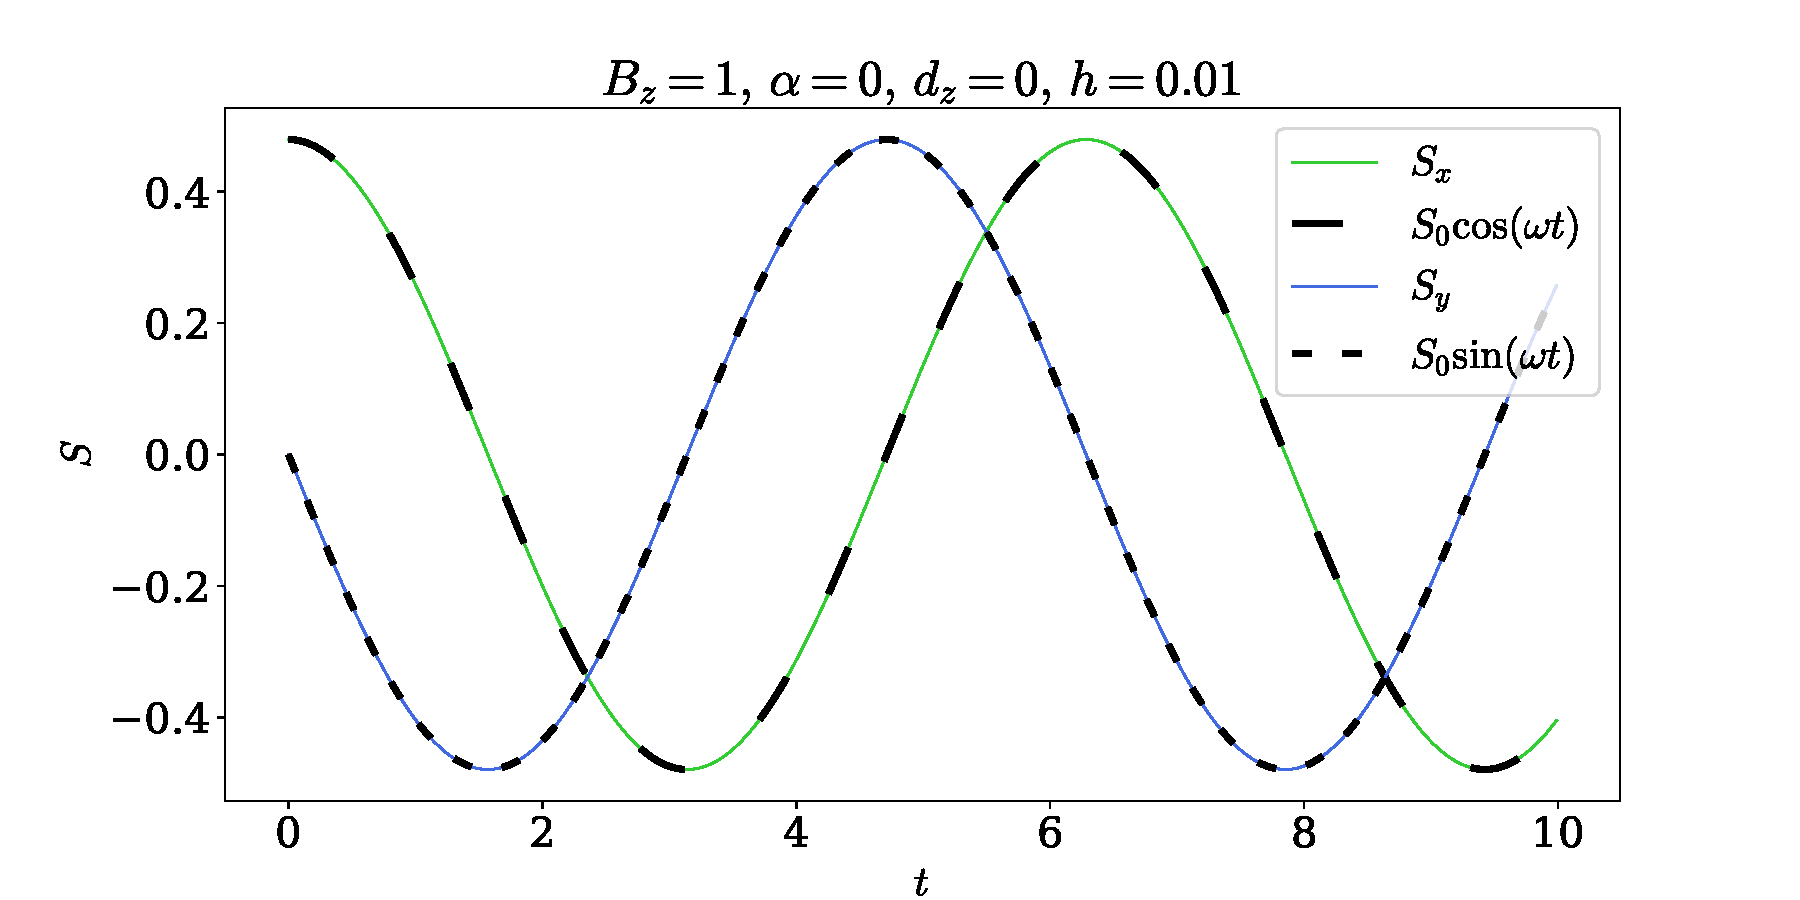
\includegraphics[width=0.8\textwidth]{../plots/single.pdf}
        \caption{caption}
        \label{single spin}
    \end{figure}

    To analyze the error, the simulation is run with differnt step lengths $h$, for the same simulation time $t_0 = 5$. The result is shown in figure \ref{error}. As Heun's method is of higher order than Euler's method, it converges faster. It is, however, necessery to make 2 function calls when using Heun's method, while Euler's method only require one. This should make Euler's method twice as fast, which was observed. Euler's method ran at around 16000 iterations per second, while Heun's method only ran at 8000. The large gain in prescision, however, makes Heun's method prefered for this application. 

    \begin{figure}
        \centering
        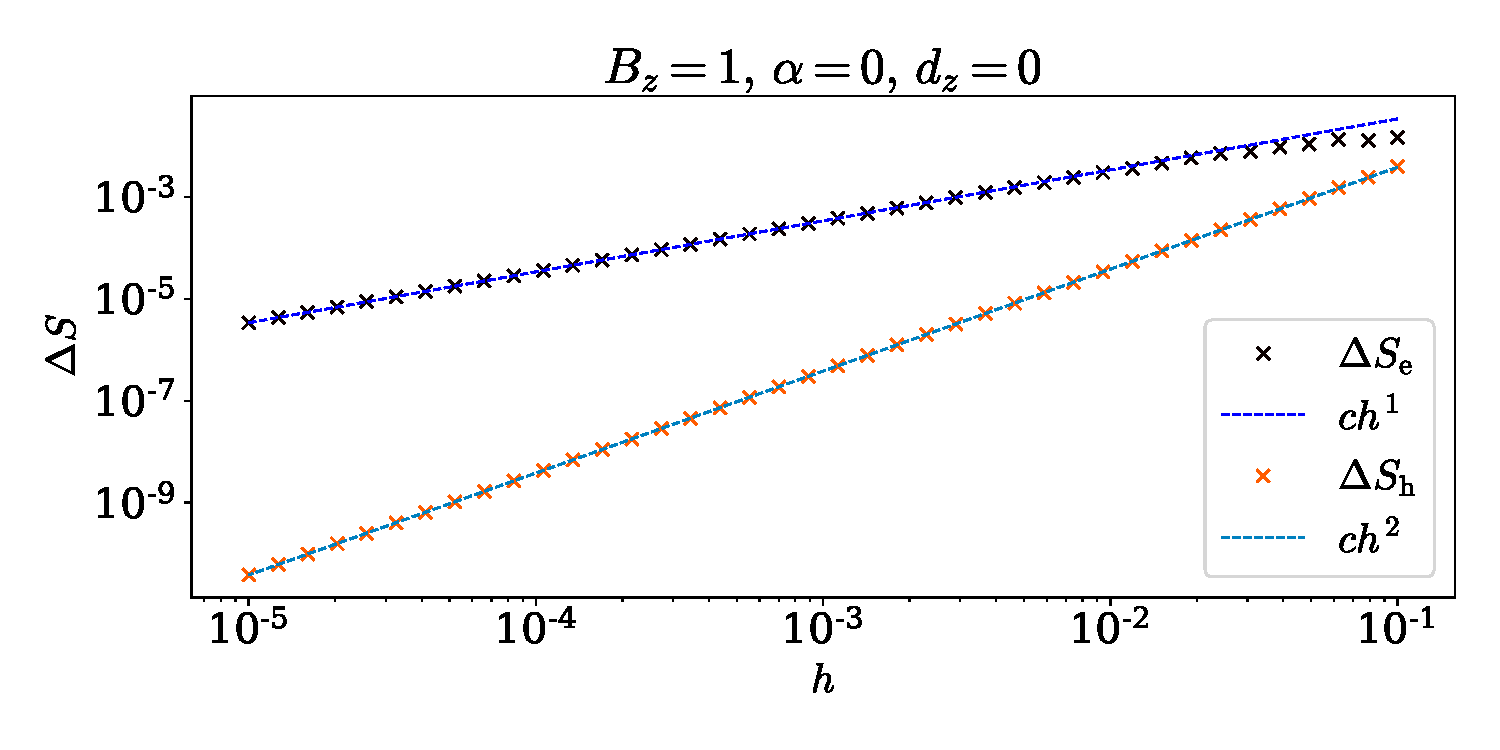
\includegraphics[width=0.8\textwidth]{../plots/err.pdf}
        \caption{caption}
        \label{error}
    \end{figure}

    When including $\alpha > 0$, one should expect the the oscillations to die away, with a lifetime given by
    \begin{equation*}
        \tau = \frac{1}{\alpha \omega}
    \end{equation*}
    Larger $\alpha$ should give a shorter lifetimes, and thus faster decay. Figure \ref{decay} shows this. Furthermore, we se that the amplitude is proportional to $\exp(-t/\tau)$. We should expect this, not only is this a common form for decay, but as no time is special, the decay should be proportional to the amplitude, which gives exponential decay.

    \begin{figure}
        \centering
        \includegraphics[width=0.33\textwidth]{../plots/decay_a=0.1.pdf}
        \includegraphics[width=0.32\textwidth]{../plots/decay_a=0.05.pdf}
        \includegraphics[width=0.33\textwidth]{../plots/decay_a=0.01.pdf}
        \caption{caption}
        \label{decay}
    \end{figure}

    \subsection*{Spin chain}
    The simulation now now includes several spins, in a ferromagnetic or anti-ferromagnetic cupling, depending on if $J = 1$ or $J = -1$, respectivley. When including damping $\alpha > 0$, both these 

    \begin{figure}
        \centering
        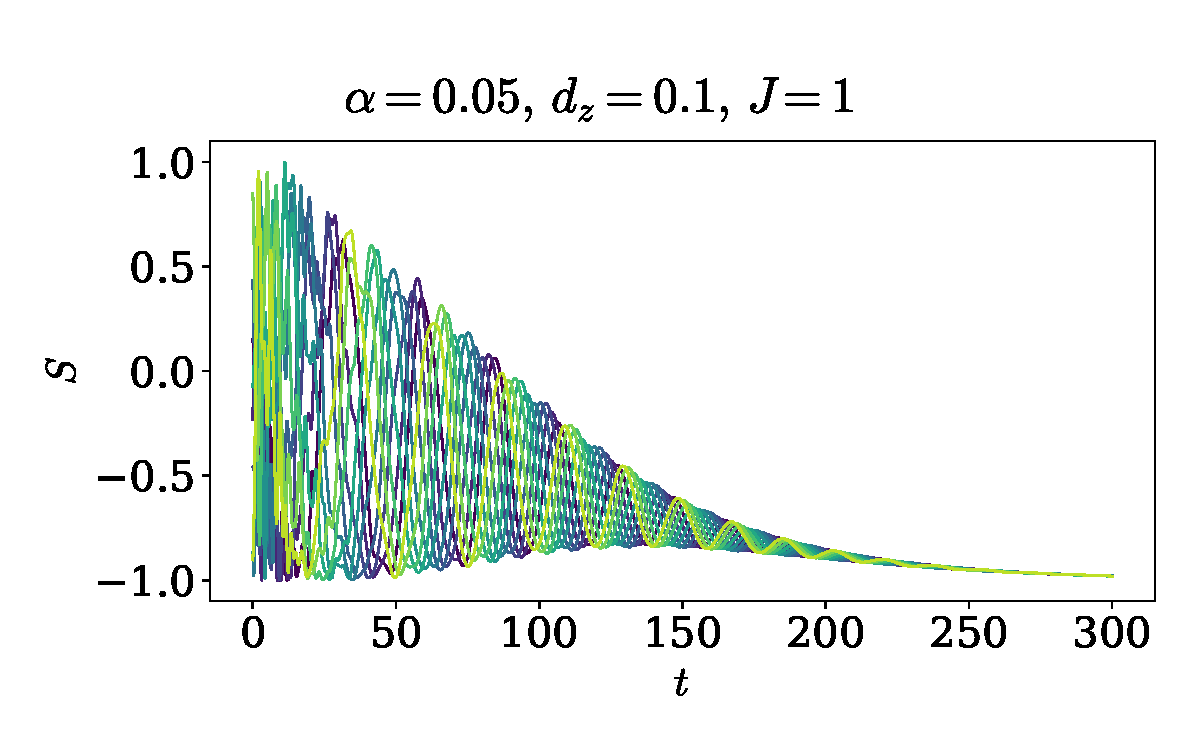
\includegraphics[width=0.49\textwidth]{../plots/ground_state_f.pdf}
        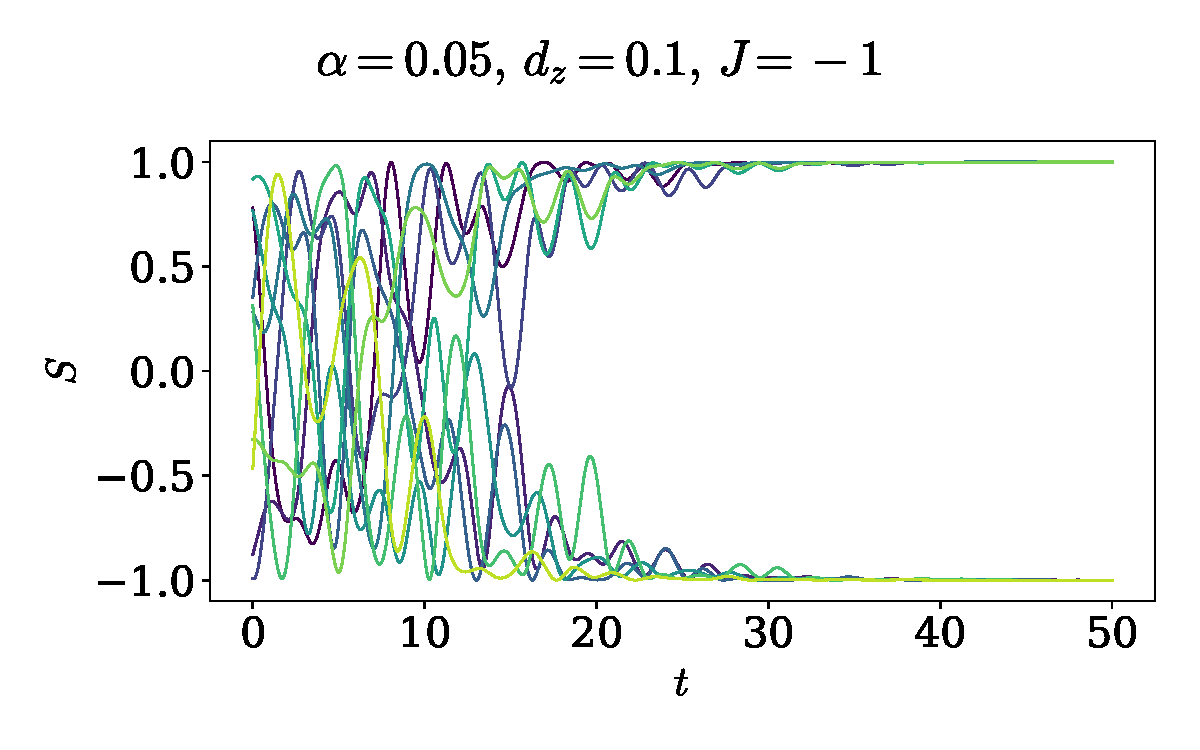
\includegraphics[width=0.49\textwidth]{../plots/ground_state_af.pdf}
        \caption{caption}
        \label{ground states}
    \end{figure}
    \begin{figure}
        \centering
        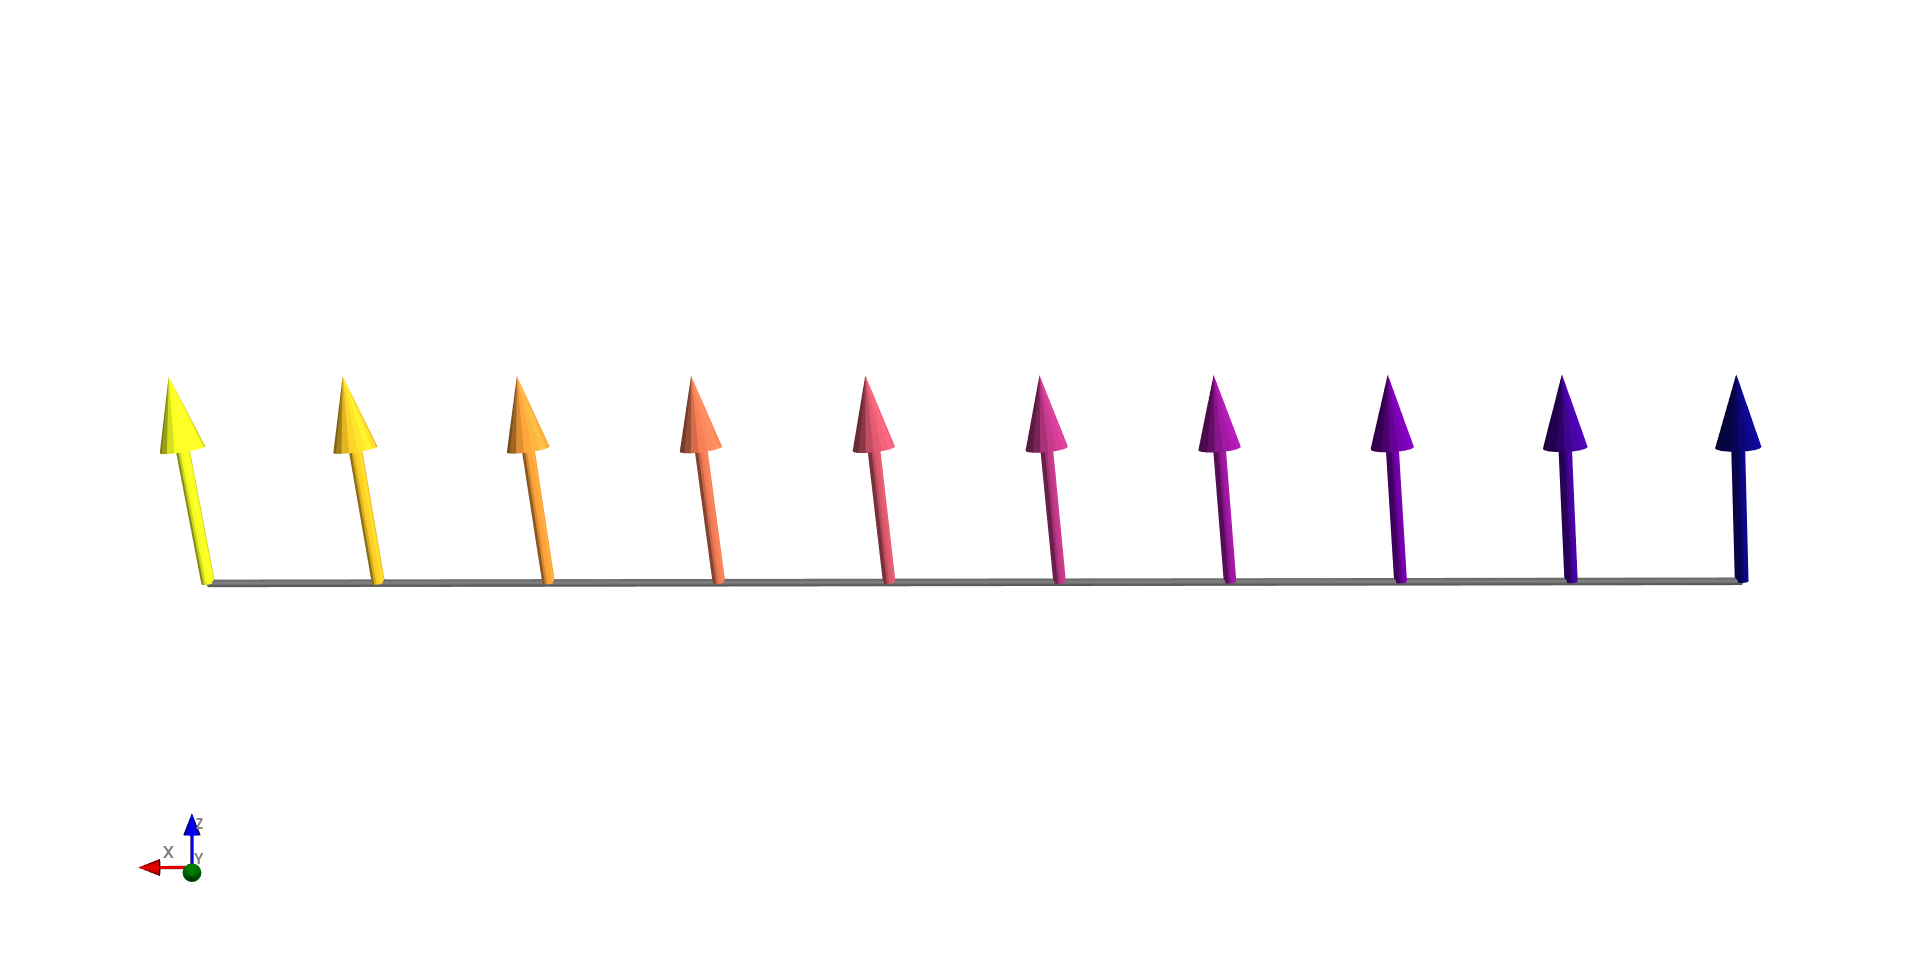
\includegraphics[width=0.49\textwidth]{../plots/ground_state_f3D.png}
        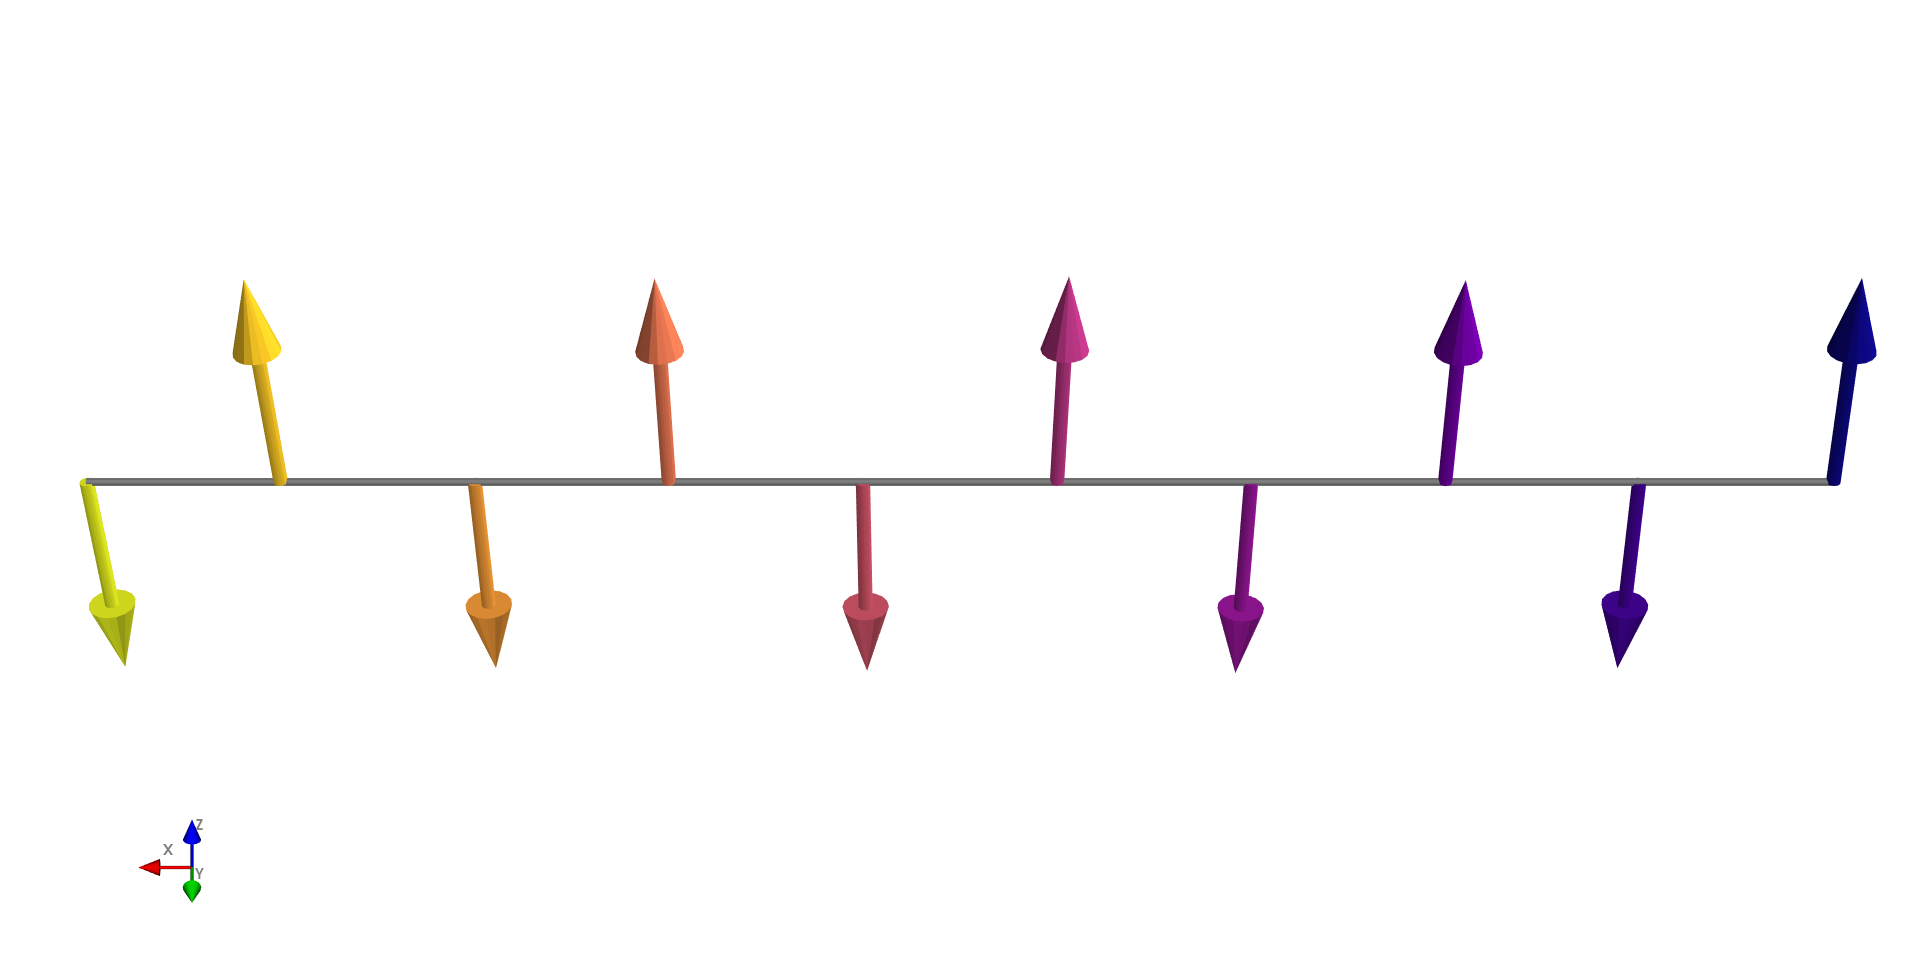
\includegraphics[width=0.49\textwidth]{../plots/ground_state_af3D.png}
        \caption{caption}
        \label{ground states}
    \end{figure}

    \bibliography{report}
    \bibliographystyle{plain}

\end{document}